\chapter{Teil1}
\label{cha:Einleitung}

\begin{normalsize}
\begin{LARGE}

\section{Motivation}
\label{sec:Motivation}

Die Bereitstellung von Wärme und elektrischer Energie beeinflusst immer stärker das Klima. Nach wie vor werden zumeist fossiler Energieträger genutzt, um den Energiebedarf zu decken. Um den Einfluss unseres Energiebedarfs auf das Klima zu reduzieren, wurden in den vergangenen Jahrzehnten verschiedene Versuche unternommen, die Energiebereitstellung auf nachhaltige Quellen umzustellen. Ziel ist insbesondere, die Anreicherung von Kohlenstoff als Kohlenstoffdioxid oder in Form anderer klimabeeinflussender Gase, wie zum Beispiel Methan, in der Atmosphäre zu verhindern. 

Die am meisten genutzten Energiequellen sind hierbei die Wasserkraft, Wind und Sonne. Dabei ist die Nutzbarkeit aller drei genannten Energiequellen stark von den geologischen, klimatischen und geographischen Bedingungen der jeweiligen Region abhängig und unterliegt in den meisten Regionen starken Leistungsschwankungen. Daher ergeben sich Probleme bei der Speicherung der Energie. Außerdem werden in den nächsten Jahren die Endenergiepreise voraussichtlich steigen, da zum einen eine Verknappung der fossilen Brennstoffe auf lange Sicht unausweichlich ist und zum anderen die Umstellung auf regenerative Energien mit einem erheblichen Kostenaufwand verbunden ist.  Deshalb haben in den letzten Jahren die Bemühungen der Politik und verschiedener Marktteilnehmer zugenommen, den Energieverbrauch zu senken. Für privat genutzte Häuser und Wohnungen geschieht das in Deutschland staatsseitig vor allem über die "Verordnung über energiesparenden Wärmeschutz und energiesparende Anlagentechnik bei Gebäuden", kurz EnEV \cite{.28.10.2015}. % [11]

Ziel der EnEV ist es, durch eine gute Dämmung den Wärmeverlust der Häuser zu reduzieren. Um entsprechende Gebäude mit ausreichend Frischluft zu versorgen, wird die Luft mittels eines Lüftungssystems ausgetauscht. Durch den Einsatz von Wärmeübertragern wird der mit dem Luftaustausch verbundene Wärmeverlust reduziert. 

Eine Konsequenz dieses Vorgehens in gemäßigten und kalten Klimaregionen ist ein Austrocknen der Raumluft. Die kalte Außenluft weist einen geringen absoluten Wassergehalt auf. Beim Erhitzen im Wärmeübertrager stellt sich so eine sehr geringe relative Feuchte ein. 
An Wohn- und Bürogebäude werden oft hohe Anforderungen bezüglich der Luftqualität gestellt. Deshalb ist es in vielen Fällen sinnvoll, die Luft auf einen Feuchtegehalt zu konditionieren, der von den Menschen als angenehm empfunden wird und keine negativen Auswirkungen auf ihren Gesundheitszustand oder ihre Leistungsfähigkeit hat. Eine detaillierte Zusammenfassung über die Auswirkungen zu trockener Luft enthält eine Publikation von Jürgen Schneiders.\cite{JurgenSchniedersDr.RainerPflugerDr.WolfgangFeist.Oktober}
%Quelle einfügen Energetische Bewertung von Wohnungslüftungsgeräten mit Feuchterückgewinnung (12)

In feucht warmen Klimazonen tritt oft ein gegenteiliger Effekt ein. Die feucht warme Zuluft wird abgekühlt und gewinnt so an relativer Feuchte. Dies kann dazu führen, dass Feuchteschäden an Bauteilen oder am Interieur des Gebäudes entstehen oder es zur Bildung von Schimmel kommt. Entsprechend ist in vielen Fällen eine Trocknung der zugeführten Luft notwendig. \cite{Zhang.2010}
%[Zhang HB and Hiroshi Y. Analysis of indoor humidity environment in Chinese residential buildings. Build Environ 2010; 45(10): 2132–2140]

In Sonderfällen ist es möglich, dass bestimmte Raumklimabedingungen eingehalten werden müssen. Zum Beispiel erfordern bestimmte Lagerbedingungen oder Rahmenbedingungen für Produktionsabläufe oder Forschungsprozesse ein definiertes Raumklima. 
Das Trocknen beziehungsweise Befeuchten der Luft kostet viel Energie. Bei einem Luftbefeuchter muss hierzu die Verdampfungsenthalpie des Wassers überwunden werden. Eine Beschreibung des Energieverbrauchs von klassisch zur Trocknung von Luft eingesetzten Sorptionstrocknern findet sich beispielsweise in \cite{Zhang.2006}
% evtl Bild für Luftbefeuchter und Sorptionstrockner
Enthalpieübertrager stellen eine Möglichkeit da, diesen Energieaufwand zu reduzieren. 

\section{Der Enthalpieübertrager}
\label{Der Enthalpieübertrager}

Aus dem Stand der Technik sind Speicherenthalpieübertrager und membranbasierte Enthalpieübertrager bekannt, wie sie in \ref{fig:Enthalpieübertrager} dargestellt sind. Beide Systeme übertragen neben Wärme auch Feuchte von einem feuchten auf einen trockenen Luftstrom. Die Triebkraft in beiden Systemen ist die Differenz des chemischen Potenzials, die ausgeglichen wird. 

\begin{figure} [h]
	%\centering
	\subfigure[Rotations, Speicherenthalpieübertrager]{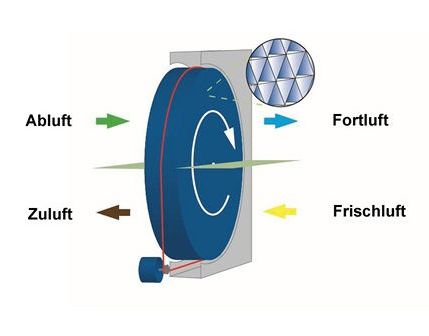
\includegraphics[width=0.49\textwidth]{Pictures/Rotation.jpg}}
	\subfigure[Membranbasierter Enthalpieübertrager]{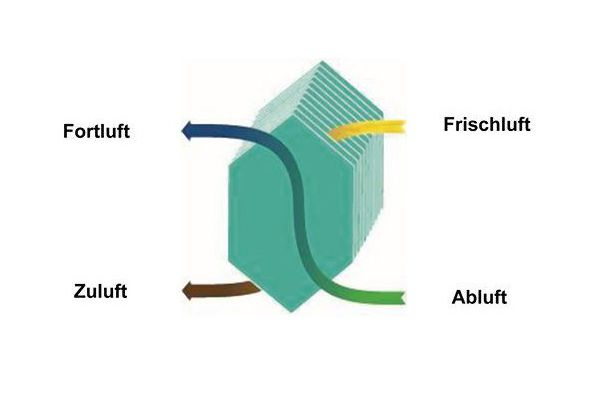
\includegraphics[width=0.49\textwidth]{Pictures/Enthalpieuebertrager.jpg}}
	\caption{Verschiedene Ausführungsformen von Enthalpieübertragern}
	\label{fig:Enthalpieübertrager}
	
\end{figure}


Die verbreitesten Speicherübertrager sind Rotationsübertrager, wie in dargestellt. Rotationsübertrager weisen eine rotierende thermische Masse auf, die sich jeweils mit einem Teil der Masse im Zuluftstrom und mit einem anderen Teil der Masse im Abluftstrom befindet. Durch die Rotation kann die Masse thermische Energie in einem Luftstrom aufnehmen und nach dem Weiterrotieren in den anderen Luftstrom abgeben. Analog funktioniert die Übertragung der Feuchte, wobei die Feuchte entweder von einem Sorptionsmaterial aufgenommen und wieder abgegeben wird oder in einem Luftstrom an der Masse kondensiert und in dem anderen Luftstrom wieder verdampft. Rotationsübertrager befinden sich bereits seit einigen Jahren kommerziell im Einsatz und wurden entsprechend detailliert untersucht. Ein detailliertes Modell von Rotationsübertagern liefert eine Untersuchng von Zhang\cite{Zhang.2002}. Die Artikel \cite{Zhang.2006} und \cite{JustoAlonso.2015} vergleichen unterschiedliche Optionen der Lufttrocknung.

Membranbasierte Enthalpieübertrager sind erst seit wenigen Jahren kommerziell im Einsatz, sodass bisher nur wenige Untersuchungen zu ihnen existieren. Die Wärme wird über die Membran von einem Luftstrom an den anderen übertragen. Analog zum übertragenen Wärmestrom wird die Feuchte übertragen. Das Wasser wird vom Membranmaterial absorbiert, diffundiert durch die Membran und desorbiert auf der anderen Seite in den Luftstrom. 

Die Geometrien, die dabei für den Enthalpieübertrager verwendet werden, entsprechen denen, die bei klassischen Wärmeübertragern zum Einsatz kommen. In kommerziellen Anwendungen kommen Kreuzstromübertrager und Kreuzgegenstromübertrager zur Anwendung. Gegenstromübertrager und "hollow fibre" Module stellen weitere mögliche Bauformen dar. Kreuzstromübertrager sind im Vergleich zu Gegenstromübertragern kostengünstig herstellbar und benötigen nur geringen Bauraum. Daher sind sie die bisher häufigste Bauform bei Enthalpietauschern. Gegenstromübertrager haben im Gegensatz dazu einen hohen Wirkungsgrad. Deshalb hält vor allem eine Mischform aus beidem, der Kreuzgegenstromübertrager, immer stärker Einzug in die kommerzielle Nutzung. Eine Darstellung der Bauweise von Hollow fibre Modulen findet sich in \ref{fig:hollow fibre Modul}. Sie ermöglichen hohe Übertragungsflächen bei kleinem Bauraum und somit hohe Übertragungsraten für Wärme und Feuchte. Dies erläutern auch die Artikel von Zhang und Bui \cite{Zhang.2010} \cite{Bui.2010}. Nachteilig ist jedoch ein sehr hoher Druckverlust in den Modulen. Der hohe Druckverlust hat bisher verhindert, dass sich diese Bauform in kommerziellen Anwendungen durchsetzen konnte. 

\begin{figure} [h]
	\centering
	%\includegraphics[width=400]{pictures/Vergleich_Geometirie.jpg}
	%\caption{Geometrien}
	%\label{fig:verschiendene Enthalpieübertrager-Geometrien}
	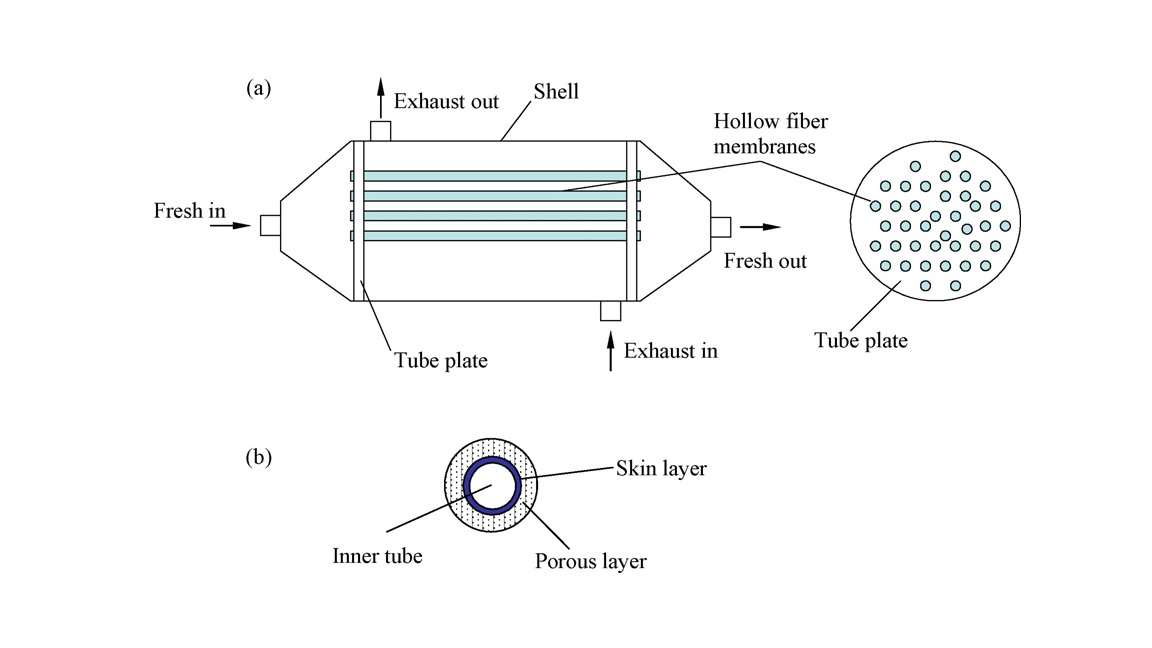
\includegraphics[width=0.98\textwidth]{pictures/hollow_fibre.jpg}
	\caption{hollow fibre}
	\label{fig:hollow fibre Modul}
\end{figure}

Ein Vergleich zwischen Rotationsübertragern und membranbasierten Enthalpietauschern fällt je nach Untersuchung unterschiedlich aus. Grundlegend haben jedoch membranbasierte Enthalpietauscher den Vorteil, dass sie keine beweglichen (rotierenden) Komponenten haben, was sie weniger verschleißanfällig macht und die Geräuschemissionen senkt. Außerdem muss keine Energie zum Antrieb eines Rotors aufgewendet werden. In den meisten Fällen besitzen membranbasierte Enthalpieübertrager den höheren Wirkungsgrad. \cite{JustoAlonso.2015}  %weitere Quelle
Nachteilig ist, dass Enthalpieübertrager nicht regelbar sind. Theoretisch
ist es daher an feucht warmen Tagen möglich, dass ein Enthalpieübertrager zur Feuchterückgewinnung der Zuluft weiter Wasser zuführt. Dann steigt die bereits hohe relative Feuchte im Gebäude weiter an. Dies könnte nur durch einen Bypass, einen Trockner oder einen temporären Austausch des Enthalpieübertragers durch einen Wärmeübertrager verhindert werden. Außerdem können die membranbasierten Übertrager bei kalten Temperaturen zufrieren und müssen daher in einigen Klimazonen mit Vorheizern ausgestattet werden. Derzeit beherrschen Rotationsübertrager vor allem den Markt bei großen Anwendungsfällen, während Enthalpieübertrager vor allem für Wohnungs- und Einzelraumlüftungen genutzt werden.  


\section{Die Membran}

Membranen lassen sich in dichte und poröse Membranen unterteilen. 
Poröse Membranen weisen Poren auf, die größer sind als die Partikel, die durch die Membran übertragen werden. In der Membrantechnik werden diese Prozesse Micro- oder Ultrafiltration genannt. Sie laufen als konvektive oder kapillare Prozesse ab. 
Dichte Membranen weisen hingegen keine oder nur sehr kleine Poren auf.  Der Stofftransport findet bei dichten Membranen auf Grund von Diffusionsprozessen statt. 
Dies führt in den meisten Fällen zu einer deutlich erhöhten Selektivität und einer geringeren Permeabilität im Vergleich zu porösen Membranen. Im vorliegenden Anwendungsfall passiert Wasserdampf als Permeat die Membran während kleine gasförmige Moleküle der Luft, wie Stickstoff, zurückgehalten werden. Daher ist eine dichte Membran sinnvoll. Nur so ist eine ausreichende Selektivität gegenüber den gasförmigen Komponenten gewährleistet. \cite{ThomasMelin.2007}
Um dennoch eine möglichst hohe Permeabilität gegenüber Wasserdampf zu gewährleisten, ist es zielführend eine möglichst dünne Membran zu verwenden. 
Die dünne dichte Membran wird in einigen Fällen durch eine poröse Membran gestützt, um diese mechanisch zu stabilisieren. Die poröse Membran hat kaum negative Auswirkungen auf die Permeabilität, da die Transportgeschwindigkeiten in porösen Membranen wesentlichen höher sind als in dichten Membranen. Gleichzeitig ist jedoch anzunehmen, dass Spacermaterialien und porösen Membranen Einfluss auf die Strömung und damit auf die Wärmeübergangskoeffizienten und Sorptionseigenschaften an der Membranoberfläche nehmen. \cite{Shrivastava.2008}  %auf wasseraffinität eingehen,

\begin{figure} [h]
	\centering
	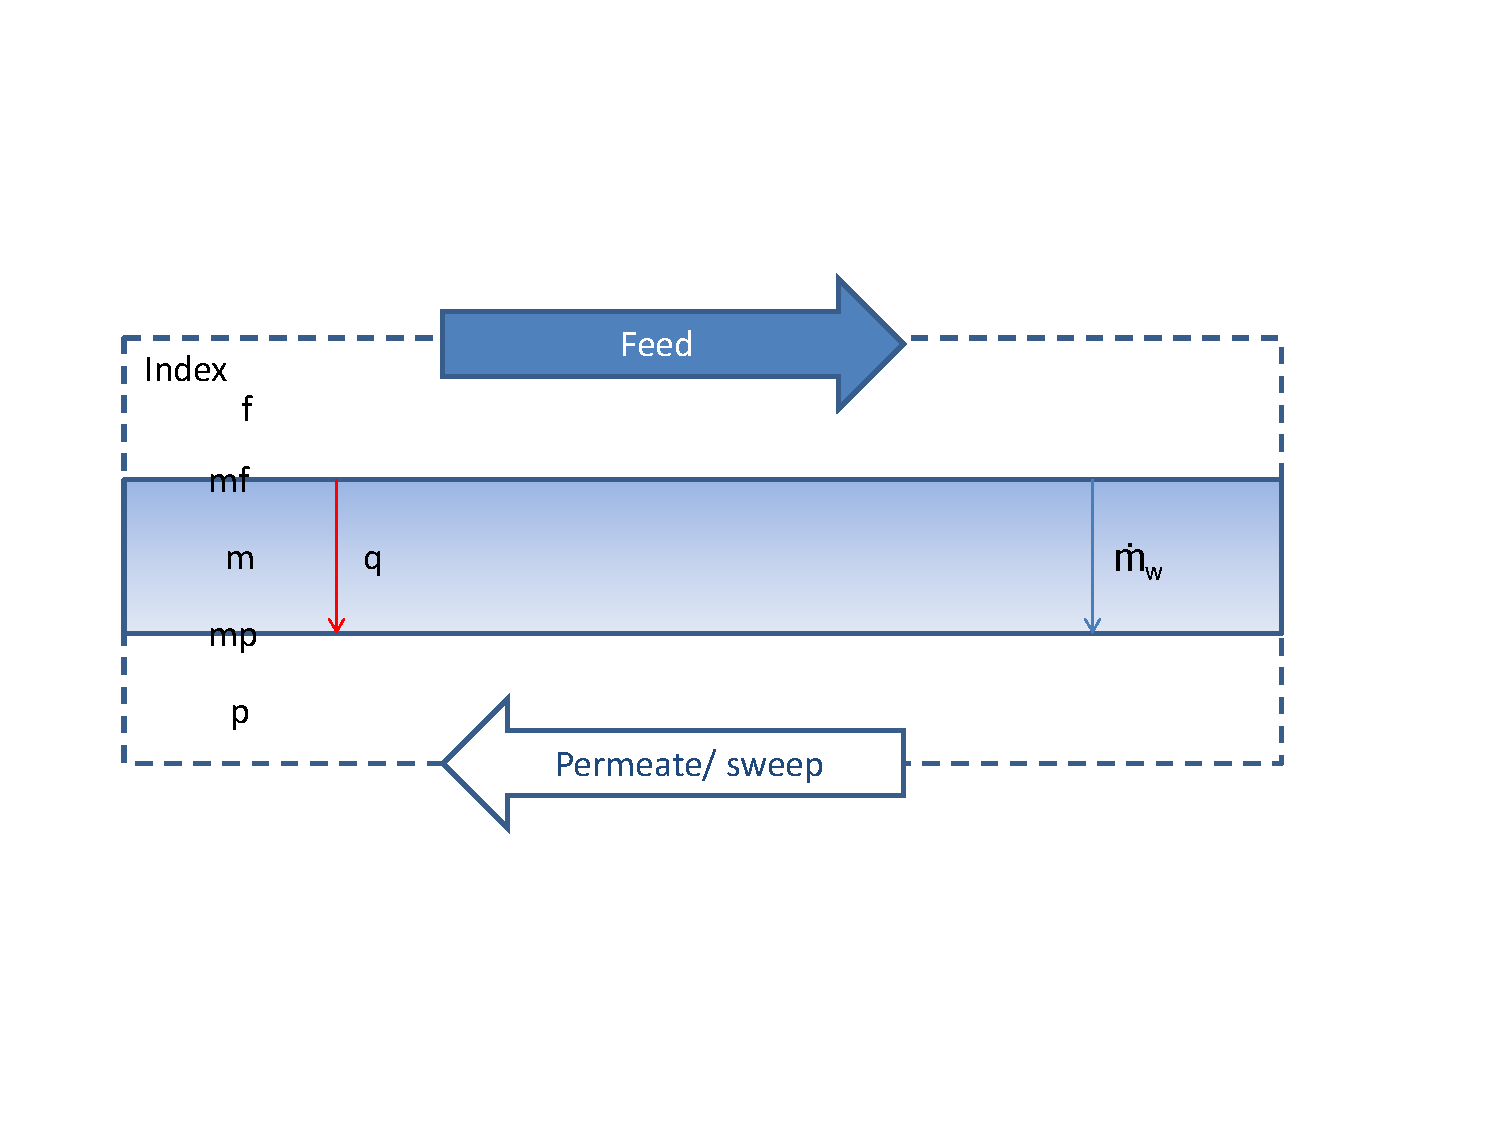
\includegraphics[width=0.98\textwidth]{pictures/Membran.pdf}
	\caption{Membran}
	\label{Membran}
\end{figure}

In Enthalpieübertragern werden derzeit Membranen aus Polymeren eingesetzt. Bis vor einigen Jahren auch wurden auch Membranen auf Zellulosebasis verwendet. Die technische Weiterentwicklung der Polymermembranen in den letzten Jahren hat dazu geführt, dass mittlerweile fast ausschließlich Polymermembranen zu Einsatz kommen, da diese deutlich höhere Permeabilitäten aufweisen. \cite{JingchunMin.}

%Der Transport des Wasser von einem Luftstrom in den anderen Luftstrom durch die Membran lässt sich in 3 Phasen einteilen. Zuerst wird das Wasser auf einer Seite von der Membran Absorbiert, dann diffundiert das flüssige Wasser durch die Membran und wird auf der anderen Seite der Membran desobiert und an den Luftstrom abgegeben. 

% bild zum Transportprozess



%Ein klassischer Vergleich über Wirkungsgrade ist nur bedingt sinnvoll. Die dabei bisher verwendeten Wirkungsgrade sind der Wärmeübertragungsgrad $\eta_{t}$ und der Enthalpiewirkungsgrad $\eta_{h}$. Der Wärmeübertragungsgrad hängt dabei allein von der thermischen Energie ab, 
%\begin{equation}

%\end{equation}.

%Der Enthalpiewirkungsgrad beschreibt die gesamte übertragene Energie, also inklusive der Enthalpie die im übertragenen Wasserdampf steckt,
%\begin{equation}

%\end{equation}

%Der Wärmeübertragungsgrad bei einem reine Wärmeübertrager ist fast immer größer, als bei einem Enthalipeübertrager und andersherum weißt der Enthalpieübertrager einen größeren gesamten Enthalpiewirkungsgrad auf.  Da membranbasierte Enthalpieübertrager ungeregelt Feuchte in den Zuluftstrom übertragen, ist die eine Bewertung anhand der Gesamtenthalpie oft nicht gerechtfertigt, da teilweise mehr Feuchte übertragen wird als benötigt. %evtl. noch auf Normzustand und Abweichung über das Jahr eingehen
%Der Wärmeübertragungsgrad stellt kein geeignetes Vergleichskriterium dar, da die übertragene Feuchte nicht berücksichtigt wird, die eine Hauptfunktion des Enthalpietauschers darstellt.




%In dieser Arbeit sollen insbesondere membranbasierte Enthalpietauscher untersucht werden und Vergleichsgrößen gefunden werden, die eine Energierückgewinnung mittels Enthalpietauschern mit anderen Systemen vergleichbar machen. Des Weiteren soll ein Modell der Enthalpieübertrager angefertigt werden, das zukünftig als Grundlage für Simulationen und für eine Weiterentwicklung der Modelle dienen soll, um Enthalpieübertrager auch in größeren Systemen simulativ einbinden zu können.  


\section{Stand der Technik}

Bisherige Veröffentlichungen beschreiben vor allem Kennzahlen und die Genauigkeit bestimmter Modell-Ansätze. Für einen Überblick über Veröffentlichungen und den derzeitigen Stand der Technik empfehlen sich vor allem die Artikel \cite{Zhang.2012} und \cite{JasonWoods.2014}.
Als Modelle werden insbesondere Lösungs-Diffusions-Modelle vorgeschlagen. Sie beruhen auf der Annahme, dass Wasserdampf an der Oberfläche der Membran absorbiert wird, durch die Membran diffundiert und auf der gegenüberliegende Seite wieder an die Luft abgegeben wird. Aus dieser Betrachtungsweise ergeben sich verschiedene Möglichkeiten, das System eines Enthalpieübertragers zu beschreiben. 
Grundsätzlich lassen sich die Publikationen in bewertungsorientierte (z.B. \cite{Nasif.2010}), komponentenoptimierungsorientierte (z.B. \cite{Chen.1997}) und modellermittelnde Untersuchungen (z.B. \cite{Zhang.2010}) unterteilen. 
Die bewertungsorientierten Arbeiten nutzen für den Vergleich verschiedener Bauweisen, Geometrien und Prinzipien bekannte Bewertungsgrößen wie den Wärmeübertragungsgrad, den Feuchteübertragungsgrad oder den totalen Enthalpieübertragungsgrad sowie die Number of transfer units.
Bisherige Untersuchungen zur Modellbildung beziehen sich weitestgehend auf die Bestimmung grundlegender Kenngrößen oder Beschreibungswerte, die analog zu bekannten Systemen definiert wurden. Der Gesamtprozess wird in Teilprozesse unterteilt, die bereits gut beschrieben sind. Auf diese Weise entstehen Modelle, die die Teilprozesse in Beziehung zueinander setzen. So lassen sich  die Strömungseigenschaften, die Wärmeübertragung und die Feuchteübertragung getrennt voneinander betrachten. Mit Kennzahlen, die ggf. von bestimmten Parametern abhängen, sind diese miteinander Verknüpfbar. 

In dieser Arbeit soll im Gegensatz dazu ein Modell eines kommerziell einsatzfähigen Enthalpieübertragers ermittelt werden. Dabei liegt der Schwerpunkt nicht auf der Ermittlung der physikalischen Grundwerte oder Gültigkeit der physikalischen Modelle  und der zu Grunde liegenden Annahmen. Stattdessen wird das Verhalten des praktisch eingesetzten Systems unter bestimmten Umgebungsbedingungen und in bestimmten Anwendungsfällen untersucht. Der Schwerpunkt liegt hier auf dem deutschen Klimaraum und dem Einsatz in Wohnraumlüftungen. 
%Die Betrachtungsweise bleibt also empirischer und und beschäftigt sich nicht mit den Materialeigenschaften
Ziel ist es, ein Modell zu generieren, das abhängig von Anforderungsprofilen und Umgebungsbedingungen eine Bewertung der Enthalpieübertrager insbesondere im Vergleich zu alternativen Systemen, wie z.B. Speicherenthalieübertragern und klassischen Wärmeübertragern mit entsprechender Lufttrocknung ermöglich. Zu diesem Zweck sollen auch Bewertungsgrößen definiert werden, die einen sinnvollen Vergleich der verschiedenen Größen zulassen. 


